\documentclass[twoside]{book}

% Packages required by doxygen
\usepackage{fixltx2e}
\usepackage{calc}
\usepackage{doxygen}
\usepackage[export]{adjustbox} % also loads graphicx
\usepackage{graphicx}
\usepackage[utf8]{inputenc}
\usepackage{makeidx}
\usepackage{multicol}
\usepackage{multirow}
\PassOptionsToPackage{warn}{textcomp}
\usepackage{textcomp}
\usepackage[nointegrals]{wasysym}
\usepackage[table]{xcolor}

% Font selection
\usepackage[T1]{fontenc}
\usepackage[scaled=.90]{helvet}
\usepackage{courier}
\usepackage{amssymb}
\usepackage{sectsty}
\renewcommand{\familydefault}{\sfdefault}
\allsectionsfont{%
  \fontseries{bc}\selectfont%
  \color{darkgray}%
}
\renewcommand{\DoxyLabelFont}{%
  \fontseries{bc}\selectfont%
  \color{darkgray}%
}
\newcommand{\+}{\discretionary{\mbox{\scriptsize$\hookleftarrow$}}{}{}}

% Page & text layout
\usepackage{geometry}
\geometry{%
  a4paper,%
  top=2.5cm,%
  bottom=2.5cm,%
  left=2.5cm,%
  right=2.5cm%
}
\tolerance=750
\hfuzz=15pt
\hbadness=750
\setlength{\emergencystretch}{15pt}
\setlength{\parindent}{0cm}
\setlength{\parskip}{0.2cm}
\makeatletter
\renewcommand{\paragraph}{%
  \@startsection{paragraph}{4}{0ex}{-1.0ex}{1.0ex}{%
    \normalfont\normalsize\bfseries\SS@parafont%
  }%
}
\renewcommand{\subparagraph}{%
  \@startsection{subparagraph}{5}{0ex}{-1.0ex}{1.0ex}{%
    \normalfont\normalsize\bfseries\SS@subparafont%
  }%
}
\makeatother

% Headers & footers
\usepackage{fancyhdr}
\pagestyle{fancyplain}
\fancyhead[LE]{\fancyplain{}{\bfseries\thepage}}
\fancyhead[CE]{\fancyplain{}{}}
\fancyhead[RE]{\fancyplain{}{\bfseries\leftmark}}
\fancyhead[LO]{\fancyplain{}{\bfseries\rightmark}}
\fancyhead[CO]{\fancyplain{}{}}
\fancyhead[RO]{\fancyplain{}{\bfseries\thepage}}
\fancyfoot[LE]{\fancyplain{}{}}
\fancyfoot[CE]{\fancyplain{}{}}
\fancyfoot[RE]{\fancyplain{}{\bfseries\scriptsize Generated on Thu Dec 17 2015 15\+:14\+:26 for Open\+Swarm by Doxygen }}
\fancyfoot[LO]{\fancyplain{}{\bfseries\scriptsize Generated on Thu Dec 17 2015 15\+:14\+:26 for Open\+Swarm by Doxygen }}
\fancyfoot[CO]{\fancyplain{}{}}
\fancyfoot[RO]{\fancyplain{}{}}
\renewcommand{\footrulewidth}{0.4pt}
\renewcommand{\chaptermark}[1]{%
  \markboth{#1}{}%
}
\renewcommand{\sectionmark}[1]{%
  \markright{\thesection\ #1}%
}

% Indices & bibliography
\usepackage{natbib}
\usepackage[titles]{tocloft}
\setcounter{tocdepth}{3}
\setcounter{secnumdepth}{5}
\makeindex

% Hyperlinks (required, but should be loaded last)
\usepackage{ifpdf}
\ifpdf
  \usepackage[pdftex,pagebackref=true]{hyperref}
\else
  \usepackage[ps2pdf,pagebackref=true]{hyperref}
\fi
\hypersetup{%
  colorlinks=true,%
  linkcolor=blue,%
  citecolor=blue,%
  unicode%
}

% Custom commands
\newcommand{\clearemptydoublepage}{%
  \newpage{\pagestyle{empty}\cleardoublepage}%
}


%===== C O N T E N T S =====

\begin{document}

% Titlepage & ToC
\hypersetup{pageanchor=false,
             bookmarks=true,
             bookmarksnumbered=true,
             pdfencoding=unicode
            }
\pagenumbering{roman}
\begin{titlepage}
\vspace*{7cm}
\begin{center}%
{\Large Open\+Swarm \\[1ex]\large 0.\+15.\+12.\+2 }\\
\vspace*{1cm}
{\large Generated by Doxygen 1.8.9.1}\\
\vspace*{0.5cm}
{\small Thu Dec 17 2015 15:14:26}\\
\end{center}
\end{titlepage}
\clearemptydoublepage
\tableofcontents
\clearemptydoublepage
\pagenumbering{arabic}
\hypersetup{pageanchor=true}

%--- Begin generated contents ---
\chapter{Open\+Swarm documentation}
\label{index}\hypertarget{index}{}\hypertarget{index_intro_sec}{}\section{Introduction}\label{index_intro_sec}
Open\+Swarm is an easy-\/to-\/use event-\/driven preemptive operating system for miniature robots. It offers abstract hardware-\/independent functions to make user code more extendible, maintainable, and portable. The hybrid kernel provides preemptive and cooperative scheduling, asynchronous programming models with events, and inter-\/process communication functions. ~\newline
~\newline
 Open\+Swarm was created during the Ph\+D of Stefan M Trenkwalder (\href{http://trenkwalder.tech}{\tt http\+://trenkwalder.\+tech}) at the University of Sheffield (\href{http://www.sheffield.ac.uk/}{\tt http\+://www.\+sheffield.\+ac.\+uk/}) under the Supervision of Dr. Roderich Gross and Dr. Andreas Kolling.

The code of Open\+Swarm can be basically divided into 3 different modules\+:
\begin{DoxyItemize}
\item Process Management
\item Event System
\item I/\+O Management (This includes device specific sensors and actuators)
\end{DoxyItemize}\hypertarget{index_brief_dec}{}\section{Documentation Structure}\label{index_brief_dec}
This documentation was generated by Doxygen (\href{http://www.doxygen.org}{\tt http\+://www.\+doxygen.\+org}) and is structured as follows
\begin{DoxyItemize}
\item Main Page\+: This tab represents an short introduction to and general comments on Open\+Swarm
\item Modules\+: This tab presents a list of logical units of Open\+Swarm (such as Process Management or Event System)
\item Data Structures\+: This tab shows a list of all used data structures inside Open\+Swarm.
\item Files\+: This tab lists the documentation of each individual file in Open\+Swarm.
\end{DoxyItemize}\hypertarget{index_LICENSE}{}\section{L\+I\+C\+E\+N\+S\+E}\label{index_LICENSE}
L\+I\+C\+E\+N\+S\+E\+: adapted Free\+B\+S\+D License Copyright (c) 2015, Stefan M. Trenkwalder All rights reserved.

Redistribution and use in source and binary forms, with or without modification, are permitted provided that the following conditions are met\+:


\begin{DoxyEnumerate}
\item Redistributions of source code must retain the above copyright notice, this list of conditions and the following disclaimer.
\item Redistributions in binary form must reproduce the above copyright notice, this list of conditions and the following disclaimer in the documentation and/or other materials provided with the distribution.
\item If this or parts of this source code (as code or binary) is, in any form, used for an commercial product or service (in any form), this product or service must provide a clear notice/message to any user/customer that Open\+Swarm was used in this product.
\end{DoxyEnumerate}

T\+H\+I\+S S\+O\+F\+T\+W\+A\+R\+E I\+S P\+R\+O\+V\+I\+D\+E\+D B\+Y T\+H\+E C\+O\+P\+Y\+R\+I\+G\+H\+T H\+O\+L\+D\+E\+R\+S A\+N\+D C\+O\+N\+T\+R\+I\+B\+U\+T\+O\+R\+S \char`\"{}\+A\+S I\+S\char`\"{} A\+N\+D A\+N\+Y E\+X\+P\+R\+E\+S\+S O\+R I\+M\+P\+L\+I\+E\+D W\+A\+R\+R\+A\+N\+T\+I\+E\+S, I\+N\+C\+L\+U\+D\+I\+N\+G, B\+U\+T N\+O\+T L\+I\+M\+I\+T\+E\+D T\+O, T\+H\+E I\+M\+P\+L\+I\+E\+D W\+A\+R\+R\+A\+N\+T\+I\+E\+S O\+F M\+E\+R\+C\+H\+A\+N\+T\+A\+B\+I\+L\+I\+T\+Y A\+N\+D F\+I\+T\+N\+E\+S\+S F\+O\+R A P\+A\+R\+T\+I\+C\+U\+L\+A\+R P\+U\+R\+P\+O\+S\+E A\+R\+E D\+I\+S\+C\+L\+A\+I\+M\+E\+D. I\+N N\+O E\+V\+E\+N\+T S\+H\+A\+L\+L T\+H\+E C\+O\+P\+Y\+R\+I\+G\+H\+T H\+O\+L\+D\+E\+R O\+R C\+O\+N\+T\+R\+I\+B\+U\+T\+O\+R\+S B\+E L\+I\+A\+B\+L\+E F\+O\+R A\+N\+Y D\+I\+R\+E\+C\+T, I\+N\+D\+I\+R\+E\+C\+T, I\+N\+C\+I\+D\+E\+N\+T\+A\+L, S\+P\+E\+C\+I\+A\+L, E\+X\+E\+M\+P\+L\+A\+R\+Y, O\+R C\+O\+N\+S\+E\+Q\+U\+E\+N\+T\+I\+A\+L D\+A\+M\+A\+G\+E\+S (I\+N\+C\+L\+U\+D\+I\+N\+G, B\+U\+T N\+O\+T L\+I\+M\+I\+T\+E\+D T\+O, P\+R\+O\+C\+U\+R\+E\+M\+E\+N\+T O\+F S\+U\+B\+S\+T\+I\+T\+U\+T\+E G\+O\+O\+D\+S O\+R S\+E\+R\+V\+I\+C\+E\+S; L\+O\+S\+S O\+F U\+S\+E, D\+A\+T\+A, O\+R P\+R\+O\+F\+I\+T\+S; O\+R B\+U\+S\+I\+N\+E\+S\+S I\+N\+T\+E\+R\+R\+U\+P\+T\+I\+O\+N) H\+O\+W\+E\+V\+E\+R C\+A\+U\+S\+E\+D A\+N\+D O\+N A\+N\+Y T\+H\+E\+O\+R\+Y O\+F L\+I\+A\+B\+I\+L\+I\+T\+Y, W\+H\+E\+T\+H\+E\+R I\+N C\+O\+N\+T\+R\+A\+C\+T, S\+T\+R\+I\+C\+T L\+I\+A\+B\+I\+L\+I\+T\+Y, O\+R T\+O\+R\+T (I\+N\+C\+L\+U\+D\+I\+N\+G N\+E\+G\+L\+I\+G\+E\+N\+C\+E O\+R O\+T\+H\+E\+R\+W\+I\+S\+E) A\+R\+I\+S\+I\+N\+G I\+N A\+N\+Y W\+A\+Y O\+U\+T O\+F T\+H\+E U\+S\+E O\+F T\+H\+I\+S S\+O\+F\+T\+W\+A\+R\+E, E\+V\+E\+N I\+F A\+D\+V\+I\+S\+E\+D O\+F T\+H\+E P\+O\+S\+S\+I\+B\+I\+L\+I\+T\+Y O\+F S\+U\+C\+H D\+A\+M\+A\+G\+E.\hypertarget{index_link_sec}{}\section{Links}\label{index_link_sec}

\begin{DoxyItemize}
\item \href{http://www.openswarm.org/}{\tt http\+://www.\+openswarm.\+org/} The official Open\+Swarm website
\item \href{http://trenkwalder.tech/}{\tt http\+://trenkwalder.\+tech/} The academic webpage of Stefan Trenkwalder
\item \href{http://naturalrobotics.group.shef.ac.uk/}{\tt http\+://naturalrobotics.\+group.\+shef.\+ac.\+uk/} The website of the research group
\item \href{http://openswarm.org/license/}{\tt http\+://openswarm.\+org/license/} The link to the newest license (in case it changed) 
\end{DoxyItemize}
\chapter{Module Index}
\section{Modules}
Here is a list of all modules\+:\begin{DoxyCompactList}
\item \contentsline{section}{Base}{\pageref{group__base}}{}
\item \contentsline{section}{Event Management}{\pageref{group__events}}{}
\item \contentsline{section}{I/\+O Management}{\pageref{group__io}}{}
\item \contentsline{section}{Shefpuck}{\pageref{group__shefpuck}}{}
\item \contentsline{section}{e-\/puck specific modules}{\pageref{group__epuck}}{}
\begin{DoxyCompactList}
\item \contentsline{section}{Camera Module}{\pageref{group__camera}}{}
\item \contentsline{section}{I2\+C interface}{\pageref{group__i2c}}{}
\item \contentsline{section}{Motor Control}{\pageref{group__motors}}{}
\item \contentsline{section}{Remote Control}{\pageref{group__remotecontrol}}{}
\item \contentsline{section}{U\+A\+R\+T 1\&2}{\pageref{group__uart}}{}
\end{DoxyCompactList}
\item \contentsline{section}{Process Manages}{\pageref{group__process}}{}
\end{DoxyCompactList}

\chapter{File Index}
\section{File List}
Here is a list of all files with brief descriptions\+:\begin{DoxyCompactList}
\item\contentsline{section}{\hyperlink{definitions_8h}{definitions.\+h} \\*This file declares general preprocessor variables and types }{\pageref{d6/dc2/definitions_8h}}{}
\item\contentsline{section}{\hyperlink{interrupts_8c}{interrupts.\+c} \\*It defines the functions to create atomic sections }{\pageref{d8/d22/interrupts_8c}}{}
\item\contentsline{section}{\hyperlink{interrupts_8h}{interrupts.\+h} \\*It declares interrupt priority levels and functions to create atomic sections }{\pageref{d6/ded/interrupts_8h}}{}
\item\contentsline{section}{\hyperlink{memory_8c}{memory.\+c} \\*Defines functions to allocate, free, and copy memory }{\pageref{df/dd5/memory_8c}}{}
\item\contentsline{section}{\hyperlink{memory_8h}{memory.\+h} \\*Declares functions to allocate, free, and copy memory }{\pageref{dc/d18/memory_8h}}{}
\item\contentsline{section}{\hyperlink{system_8c}{system.\+c} \\*Defines functions to initialise and start Open\+Swarm }{\pageref{d4/dfd/system_8c}}{}
\item\contentsline{section}{\hyperlink{system_8h}{system.\+h} \\*Declares functions to initialise and start Open\+Swarm }{\pageref{dc/db2/system_8h}}{}
\item\contentsline{section}{events/\hyperlink{events_8c}{events.\+c} \\*Defines functions to create, (un)subscribe, (un)register, and delete events and related handler }{\pageref{de/deb/events_8c}}{}
\item\contentsline{section}{events/\hyperlink{events_8h}{events.\+h} \\*Declares functions to create, (un)subscribe, (un)register, and delete events and related handler }{\pageref{db/dd2/events_8h}}{}
\item\contentsline{section}{io/\hyperlink{io_8c}{io.\+c} \\*Defines functions to control the I\+O timer and to (un)register I\+O Handler }{\pageref{df/d0a/io_8c}}{}
\item\contentsline{section}{io/\hyperlink{io_8h}{io.\+h} \\*Declares functions to control the I\+O timer and to (un)register I\+O Handler }{\pageref{dc/dac/io_8h}}{}
\item\contentsline{section}{io/\hyperlink{io__clock_8c}{io\+\_\+clock.\+c} \\*Defines the system clock that provides a continuous time value (granulation of 1 ms) }{\pageref{da/d17/io__clock_8c}}{}
\item\contentsline{section}{io/\hyperlink{io__clock_8h}{io\+\_\+clock.\+h} \\*Declares the system clock that provides a continuous time value (granulation of 1 ms) }{\pageref{d9/ded/io__clock_8h}}{}
\item\contentsline{section}{platform/e-\/puck/\hyperlink{camera_8c}{camera.\+c} \\*This file includes functions to process data retrieved by a camera }{\pageref{d1/de0/camera_8c}}{}
\item\contentsline{section}{platform/e-\/puck/\hyperlink{camera_8h}{camera.\+h} \\*This file includes functions to process data retrieved by a camera }{\pageref{d7/df6/camera_8h}}{}
\item\contentsline{section}{platform/e-\/puck/\hyperlink{camera__processing_8c}{camera\+\_\+processing.\+c} }{\pageref{df/ded/camera__processing_8c}}{}
\item\contentsline{section}{platform/e-\/puck/\hyperlink{camera__processing_8h}{camera\+\_\+processing.\+h} }{\pageref{d6/d91/camera__processing_8h}}{}
\item\contentsline{section}{platform/e-\/puck/\hyperlink{DSPIC30F6014A__HDI_8h}{D\+S\+P\+I\+C30\+F6014\+A\+\_\+\+H\+D\+I.\+h} \\*Declares e-\/puck specific types and preprocessor variables }{\pageref{d9/d1f/DSPIC30F6014A__HDI_8h}}{}
\item\contentsline{section}{platform/e-\/puck/\hyperlink{i2c_8c}{i2c.\+c} \\*Defines functions to read and write on the I2\+C interface }{\pageref{d9/dcb/i2c_8c}}{}
\item\contentsline{section}{platform/e-\/puck/\hyperlink{i2c_8h}{i2c.\+h} \\*This file includes functions to read and write on the I2\+C interface }{\pageref{d5/daf/i2c_8h}}{}
\item\contentsline{section}{platform/e-\/puck/\hyperlink{i2c__data_8c}{i2c\+\_\+data.\+c} \\*Defines functions to manage the I2\+C queue }{\pageref{df/dd6/i2c__data_8c}}{}
\item\contentsline{section}{platform/e-\/puck/\hyperlink{i2c__data_8h}{i2c\+\_\+data.\+h} \\*This file includes functions to read and write on the I2\+C interface }{\pageref{d8/ded/i2c__data_8h}}{}
\item\contentsline{section}{platform/e-\/puck/\hyperlink{i2c__HDI_8c}{i2c\+\_\+\+H\+D\+I.\+c} \\*Hardware dependent implementations to read and write on the I2\+C interface }{\pageref{d9/df1/i2c__HDI_8c}}{}
\item\contentsline{section}{platform/e-\/puck/\hyperlink{i2c__HDI_8h}{i2c\+\_\+\+H\+D\+I.\+h} \\*Hardware dependent implementations to read and write on the I2\+C interface }{\pageref{d4/db3/i2c__HDI_8h}}{}
\item\contentsline{section}{platform/e-\/puck/\hyperlink{io__HDI_8c}{io\+\_\+\+H\+D\+I.\+c} \\*Hardware dependent implementations to start and stop the I/\+O timer. This timer executes I\+O functions periodically }{\pageref{d3/d87/io__HDI_8c}}{}
\item\contentsline{section}{platform/e-\/puck/\hyperlink{io__HDI_8h}{io\+\_\+\+H\+D\+I.\+h} \\*Hardware dependent implementations to start and stop the I/\+O timer. This timer executes I\+O functions periodically }{\pageref{d1/d81/io__HDI_8h}}{}
\item\contentsline{section}{platform/e-\/puck/\hyperlink{motors_8c}{motors.\+c} \\*This file provides the function needed to actuate the motors }{\pageref{d6/d0e/motors_8c}}{}
\item\contentsline{section}{platform/e-\/puck/\hyperlink{motors_8h}{motors.\+h} \\*This file provides the function needed to actuate the motors }{\pageref{dd/d59/motors_8h}}{}
\item\contentsline{section}{platform/e-\/puck/\hyperlink{motors__HDI_8c}{motors\+\_\+\+H\+D\+I.\+c} \\*Hardware dependent implementations to actuate the motors }{\pageref{da/d9d/motors__HDI_8c}}{}
\item\contentsline{section}{platform/e-\/puck/\hyperlink{motors__HDI_8h}{motors\+\_\+\+H\+D\+I.\+h} \\*Hardware dependent implementations to actuate the motors }{\pageref{df/d85/motors__HDI_8h}}{}
\item\contentsline{section}{platform/e-\/puck/\hyperlink{process__Management__HDI_8c}{process\+\_\+\+Management\+\_\+\+H\+D\+I.\+c} \\*Hardware dependent implementations to manage processes (e.\+g. task swichting) }{\pageref{d2/d78/process__Management__HDI_8c}}{}
\item\contentsline{section}{platform/e-\/puck/\hyperlink{process__Management__HDI_8h}{process\+\_\+\+Management\+\_\+\+H\+D\+I.\+h} \\*Hardware dependent implementations to manage processes (e.\+g. task swichting) }{\pageref{de/dad/process__Management__HDI_8h}}{}
\item\contentsline{section}{platform/e-\/puck/\hyperlink{remoteControl_8c}{remote\+Control.\+c} \\*This file includes functions needed to receive and decode messages from a remote control }{\pageref{d7/d92/remoteControl_8c}}{}
\item\contentsline{section}{platform/e-\/puck/\hyperlink{remoteControl_8h}{remote\+Control.\+h} \\*This file includes functions needed to receive and decode messages from a remote control }{\pageref{d2/d2f/remoteControl_8h}}{}
\item\contentsline{section}{platform/e-\/puck/\hyperlink{remoteControl__HDI_8c}{remote\+Control\+\_\+\+H\+D\+I.\+c} \\*Hardware dependent implementations to receive and decode messages from a remote control }{\pageref{d0/dae/remoteControl__HDI_8c}}{}
\item\contentsline{section}{platform/e-\/puck/\hyperlink{remoteControl__HDI_8h}{remote\+Control\+\_\+\+H\+D\+I.\+h} \\*Hardware dependent implementations to receive and decode messages from a remote control }{\pageref{d8/d4a/remoteControl__HDI_8h}}{}
\item\contentsline{section}{platform/e-\/puck/\hyperlink{system__Timer__HDI_8c}{system\+\_\+\+Timer\+\_\+\+H\+D\+I.\+c} \\*Hardware dependent implementations to initialise, configure and the operating system }{\pageref{d7/de8/system__Timer__HDI_8c}}{}
\item\contentsline{section}{platform/e-\/puck/\hyperlink{system__Timer__HDI_8h}{system\+\_\+\+Timer\+\_\+\+H\+D\+I.\+h} \\*Hardware dependent implementations to initialise, configure and the operating system }{\pageref{d7/d30/system__Timer__HDI_8h}}{}
\item\contentsline{section}{platform/e-\/puck/\hyperlink{traps_8c}{traps.\+c} \\*Hardware dependent implementations to catch hardware traps }{\pageref{d8/d4b/traps_8c}}{}
\item\contentsline{section}{platform/e-\/puck/\hyperlink{uart_8c}{uart.\+c} \\*This file includes functions needed to transmit data via uart(1 \& 2) }{\pageref{d1/d87/uart_8c}}{}
\item\contentsline{section}{platform/e-\/puck/\hyperlink{uart_8h}{uart.\+h} \\*This file includes functions needed to transmit data via uart(1 \& 2) }{\pageref{d2/d86/uart_8h}}{}
\item\contentsline{section}{platform/e-\/puck/\hyperlink{uart__HDI_8c}{uart\+\_\+\+H\+D\+I.\+c} \\*Hardware dependent implementations to control the message flow of the U\+A\+R\+T interface }{\pageref{da/d3a/uart__HDI_8c}}{}
\item\contentsline{section}{platform/e-\/puck/\hyperlink{uart__HDI_8h}{uart\+\_\+\+H\+D\+I.\+h} \\*Hardware dependent implementations to control the message flow of the U\+A\+R\+T interface }{\pageref{dc/d0b/uart__HDI_8h}}{}
\item\contentsline{section}{processes/\hyperlink{data_8c}{data.\+c} \\*This file includes all functions which are needed to manage data structures needed by the processes management }{\pageref{de/da9/data_8c}}{}
\item\contentsline{section}{processes/\hyperlink{data_8h}{data.\+h} \\*This file includes all functions which are needed to manage data structures needed by the processes management }{\pageref{d2/dbd/data_8h}}{}
\item\contentsline{section}{processes/\hyperlink{process__Management_8c}{process\+\_\+\+Management.\+c} \\*This file includes all functions wich are needed to manage processes (e.\+g. task swichting) }{\pageref{da/d14/process__Management_8c}}{}
\item\contentsline{section}{processes/\hyperlink{process__Management_8h}{process\+\_\+\+Management.\+h} \\*This file includes all functions wich are needed to manage processes (e.\+g. task creation, switching, termination) }{\pageref{dd/de5/process__Management_8h}}{}
\item\contentsline{section}{processes/\hyperlink{scheduler_8c}{scheduler.\+c} \\*This file includes all functions wich are needed to specify a scheduling algorithm }{\pageref{dd/d6c/scheduler_8c}}{}
\item\contentsline{section}{processes/\hyperlink{scheduler_8h}{scheduler.\+h} \\*This file includes all functions wich are needed to specify a scheduling algorithm }{\pageref{d2/dd8/scheduler_8h}}{}
\item\contentsline{section}{processes/\hyperlink{system__Timer_8c}{system\+\_\+\+Timer.\+c} \\*This file includes all hardware dependent functions, which are nesessary to initialise, configure and run the system Time }{\pageref{de/dfb/system__Timer_8c}}{}
\item\contentsline{section}{processes/\hyperlink{system__Timer_8h}{system\+\_\+\+Timer.\+h} \\*This file includes all hardware dependent functions, which are nesessary to initialise, configure and run the system Time }{\pageref{df/dbf/system__Timer_8h}}{}
\end{DoxyCompactList}

\chapter{Module Documentation}
\hypertarget{group__base}{}\subsection{Kernel}
\label{group__base}\index{Kernel@{Kernel}}


Open\+Swarm provides functions to start and initialise the operating system; allocate, free and copy memory; and create and end atomic sections.  


\subsubsection*{Files}
\begin{DoxyCompactItemize}
\item 
file \hyperlink{interrupts_8c}{interrupts.\+c}
\begin{DoxyCompactList}\small\item\em It defines the functions to create atomic sections. \end{DoxyCompactList}\item 
file \hyperlink{interrupts_8h}{interrupts.\+h}
\begin{DoxyCompactList}\small\item\em It declares interrupt priority levels and functions to create atomic sections. \end{DoxyCompactList}\item 
file \hyperlink{memory_8c}{memory.\+c}
\begin{DoxyCompactList}\small\item\em It defines functions to allocate, free, and copy memory. \end{DoxyCompactList}\item 
file \hyperlink{memory_8h}{memory.\+h}
\begin{DoxyCompactList}\small\item\em It declares functions to allocate, free, and copy memory. \end{DoxyCompactList}\item 
file \hyperlink{system_8c}{system.\+c}
\begin{DoxyCompactList}\small\item\em defines functions to initialise and start Open\+Swarm. \end{DoxyCompactList}\item 
file \hyperlink{system_8h}{system.\+h}
\begin{DoxyCompactList}\small\item\em It declares functions to initialise and start Open\+Swarm. \end{DoxyCompactList}\end{DoxyCompactItemize}


\subsubsection{Detailed Description}
Open\+Swarm provides functions to start and initialise the operating system; allocate, free and copy memory; and create and end atomic sections. 

\begin{DoxyAuthor}{Author}
Stefan M. Trenkwalder \href{mailto:s.trenkwalder@openswarm.org}{\tt s.\+trenkwalder@openswarm.\+org}
\end{DoxyAuthor}
\hypertarget{group__base_sec_intro_base}{}\subsubsection{Introduction}\label{group__base_sec_intro_base}
The Kernel contains basic functions to initialise and start all modules of Open\+Swarm. This part of Open\+Swarm executes all three modules
\begin{DoxyEnumerate}
\item \hyperlink{group__process}{Process Management}
\item \hyperlink{group__events}{Event Management}
\item \hyperlink{group__io}{I/\+O Management}
\end{DoxyEnumerate}

First, the system has to be configured by setting preprocessor values and variables. Then, Open\+Swarm initialises the system and I/\+O according to its configuration (preprocessor definitions) and with an additional command the system can be started. In addition, functions to define atomic sections (sections that cannot be interrupted by anything), allocate and free memory are also provided.\hypertarget{group__base_ssec_intro_base_defs}{}\paragraph{Definitions}\label{group__base_ssec_intro_base_defs}
definition.\+h provides standardised ports, configures the used platform, and defines general preprocessor/type definitions that are needed in Open\+Swarm.\hypertarget{group__base_ssec_intro_base_mem}{}\paragraph{Memory Management}\label{group__base_ssec_intro_base_mem}
Open\+Swarm is designed for processing units that lack a M\+M\+U (Memory Management Unit). As a consequence, advance memory management functions as virtual memory cannot be implemented without a significant reduction of efficiency.

However, Open\+Swarm provides atomic functions to allocate, free and copy memory in \hyperlink{memory_8h}{memory.\+h}.\hypertarget{group__base_ssec_intro_base_irq}{}\paragraph{Interrupt Management}\label{group__base_ssec_intro_base_irq}
Open\+Swarm provides defined interrupt priorities and functions to create atomic sections in \hyperlink{interrupts_8h}{interrupts.\+h}. A atomic section is a section of code that cannot be interrupted. 
\chapter{File Documentation}
\hypertarget{definitions_8h}{}\section{definitions.\+h File Reference}
\label{definitions_8h}\index{definitions.\+h@{definitions.\+h}}
{\ttfamily \#include $<$stdbool.\+h$>$}\\*
{\ttfamily \#include $<$stdint.\+h$>$}\\*
{\ttfamily \#include $<$p30\+F6014\+A.\+h$>$}\\*
{\ttfamily \#include \char`\"{}platform/e-\/puck/library/motor\+\_\+led/e\+\_\+epuck\+\_\+ports.\+h\char`\"{}}\\*
Include dependency graph for definitions.\+h\+:

\hypertarget{interrupts_8c}{}\section{interrupts.\+c File Reference}
\label{interrupts_8c}\index{interrupts.\+c@{interrupts.\+c}}


It defines the functions to create atomic sections.  


{\ttfamily \#include \char`\"{}interrupts.\+h\char`\"{}}\\*
{\ttfamily \#include \char`\"{}definitions.\+h\char`\"{}}\\*
Include dependency graph for interrupts.\+c\+:
\nopagebreak
\begin{figure}[H]
\begin{center}
\leavevmode
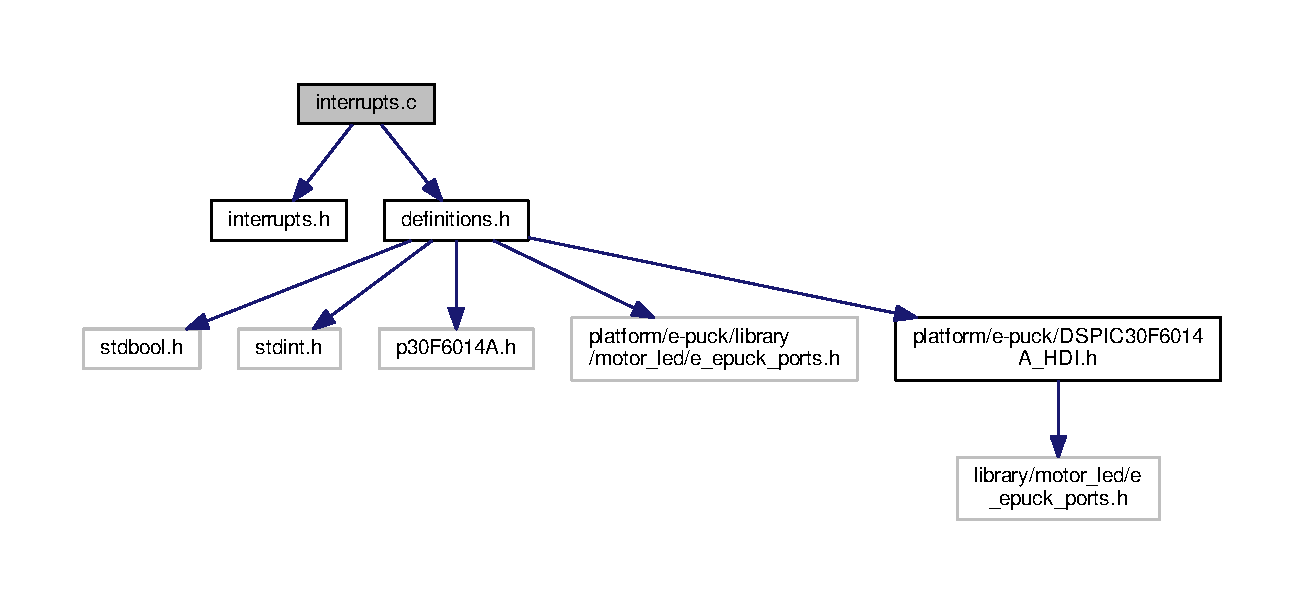
\includegraphics[width=350pt]{d3/d24/interrupts_8c__incl}
\end{center}
\end{figure}
\subsection*{Functions}
\begin{DoxyCompactItemize}
\item 
void \hyperlink{interrupts_8c_acce68565a1263b2b7bc870bfe0601f45}{Sys\+\_\+\+Start\+\_\+\+Atomic\+Section} ()
\item 
void \hyperlink{interrupts_8c_a04cce7e66e6b181477698c6398714240}{Sys\+\_\+\+End\+\_\+\+Atomic\+Section} ()
\end{DoxyCompactItemize}


\subsection{Detailed Description}
It defines the functions to create atomic sections. 

\begin{DoxyAuthor}{Author}
Stefan M. Trenkwalder \href{mailto:s.trenkwalder@openswarm.org}{\tt s.\+trenkwalder@openswarm.\+org} 
\end{DoxyAuthor}
\begin{DoxyVersion}{Version}
1.\+0 
\end{DoxyVersion}
\begin{DoxyDate}{Date}
2015 
\end{DoxyDate}
\begin{DoxyCopyright}{Copyright}
adapted Free\+B\+S\+D License (see \href{http://openswarm.org/license}{\tt http\+://openswarm.\+org/license})
\end{DoxyCopyright}
~\newline
 To protect sections of code from any interruptions one has to use the following code\+: 
\begin{DoxyCode}
\textcolor{comment}{// do something}

\hyperlink{interrupts_8c_acce68565a1263b2b7bc870bfe0601f45}{Sys\_Start\_AtomicSection}();
     
     \textcolor{comment}{//do something which should not be interrupted     }

\hyperlink{interrupts_8c_a04cce7e66e6b181477698c6398714240}{Sys\_End\_AtomicSection}();

\textcolor{comment}{// do something else}
\end{DoxyCode}
 

\subsection{Function Documentation}
\hypertarget{interrupts_8c_a04cce7e66e6b181477698c6398714240}{}\index{interrupts.\+c@{interrupts.\+c}!Sys\+\_\+\+End\+\_\+\+Atomic\+Section@{Sys\+\_\+\+End\+\_\+\+Atomic\+Section}}
\index{Sys\+\_\+\+End\+\_\+\+Atomic\+Section@{Sys\+\_\+\+End\+\_\+\+Atomic\+Section}!interrupts.\+c@{interrupts.\+c}}
\subsubsection[{Sys\+\_\+\+End\+\_\+\+Atomic\+Section}]{\setlength{\rightskip}{0pt plus 5cm}void Sys\+\_\+\+End\+\_\+\+Atomic\+Section (
\begin{DoxyParamCaption}
\item[{void}]{}
\end{DoxyParamCaption}
)\hspace{0.3cm}{\ttfamily [inline]}}\label{interrupts_8c_a04cce7e66e6b181477698c6398714240}
Starts an atomic section

This Function starts an atomic section. This means the code afterwards cannot be interrupted by any interrupt. \begin{DoxyPrecond}{Precondition}
\hyperlink{interrupts_8c_acce68565a1263b2b7bc870bfe0601f45}{Sys\+\_\+\+Start\+\_\+\+Atomic\+Section()} must have been called. 
\end{DoxyPrecond}


Definition at line 58 of file interrupts.\+c.

\hypertarget{interrupts_8c_acce68565a1263b2b7bc870bfe0601f45}{}\index{interrupts.\+c@{interrupts.\+c}!Sys\+\_\+\+Start\+\_\+\+Atomic\+Section@{Sys\+\_\+\+Start\+\_\+\+Atomic\+Section}}
\index{Sys\+\_\+\+Start\+\_\+\+Atomic\+Section@{Sys\+\_\+\+Start\+\_\+\+Atomic\+Section}!interrupts.\+c@{interrupts.\+c}}
\subsubsection[{Sys\+\_\+\+Start\+\_\+\+Atomic\+Section}]{\setlength{\rightskip}{0pt plus 5cm}void Sys\+\_\+\+Start\+\_\+\+Atomic\+Section (
\begin{DoxyParamCaption}
\item[{void}]{}
\end{DoxyParamCaption}
)\hspace{0.3cm}{\ttfamily [inline]}}\label{interrupts_8c_acce68565a1263b2b7bc870bfe0601f45}
Starts an atomic section

This Function starts an atomic section. This means the code afterwards cannot be interrupted by any interrupt. \begin{DoxyNote}{Note}
This function can be called within an atomic section. However, it doesn\textquotesingle{}t change the behaviour when called within an atomic section. To end an atomic section, \hyperlink{interrupts_8c_a04cce7e66e6b181477698c6398714240}{Sys\+\_\+\+End\+\_\+\+Atomic\+Section()} must be called as often as \hyperlink{interrupts_8c_acce68565a1263b2b7bc870bfe0601f45}{Sys\+\_\+\+Start\+\_\+\+Atomic\+Section()} was called. 
\end{DoxyNote}
\begin{DoxyPostcond}{Postcondition}
\hyperlink{interrupts_8c_a04cce7e66e6b181477698c6398714240}{Sys\+\_\+\+End\+\_\+\+Atomic\+Section()} must be called to execute any interrupt that happened or will happen. 
\end{DoxyPostcond}


Definition at line 43 of file interrupts.\+c.


\hypertarget{interrupts_8h}{}\section{interrupts.\+h File Reference}
\label{interrupts_8h}\index{interrupts.\+h@{interrupts.\+h}}


It declares interrupt priority levels and functions to create atomic sections.  


This graph shows which files directly or indirectly include this file\+:
\nopagebreak
\begin{figure}[H]
\begin{center}
\leavevmode
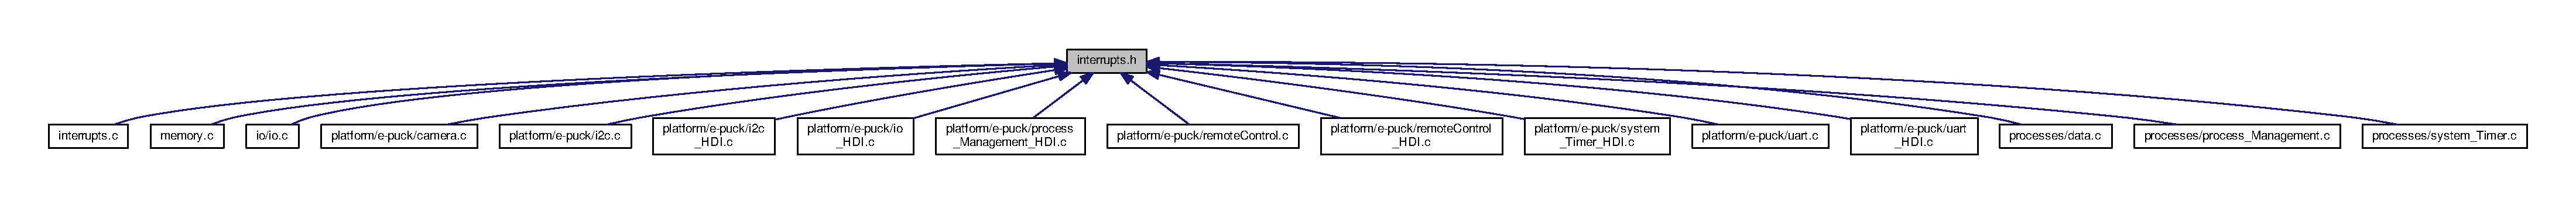
\includegraphics[width=350pt]{d9/d4e/interrupts_8h__dep__incl}
\end{center}
\end{figure}
\subsection*{Macros}
\begin{DoxyCompactItemize}
\item 
\#define \hyperlink{interrupts_8h_a2665dac9b4f047c8d82e7076eb2c1f0b}{S\+Y\+S\+\_\+\+I\+R\+Q\+P\+\_\+\+M\+A\+X}~7
\item 
\#define \hyperlink{interrupts_8h_ae792a67469dbfd96699107868d70b89d}{S\+Y\+S\+\_\+\+I\+R\+Q\+P\+\_\+\+S\+Y\+S\+T\+E\+M\+\_\+\+T\+I\+M\+E\+R}~2
\item 
\#define \hyperlink{interrupts_8h_acea06e741c8e65e966768399b39550fd}{S\+Y\+S\+\_\+\+I\+R\+Q\+P\+\_\+\+I\+O\+\_\+\+T\+I\+M\+E\+R}~3
\item 
\#define \hyperlink{interrupts_8h_a20e8d0849325b72878dc32b27876a07b}{S\+Y\+S\+\_\+\+I\+R\+Q\+P\+\_\+\+U\+A\+R\+T1}~4
\item 
\#define \hyperlink{interrupts_8h_a8a1e0a0bb08cf252f8ffe0d80f04cf49}{S\+Y\+S\+\_\+\+I\+R\+Q\+P\+\_\+\+U\+A\+R\+T2}~4
\item 
\#define \hyperlink{interrupts_8h_abe88b597dc055319b1224b2bfda0ed78}{S\+Y\+S\+\_\+\+I\+R\+Q\+P\+\_\+\+I2\+C}~5
\item 
\#define \hyperlink{interrupts_8h_a8861626b5e152d2faca2df0622c0d48e}{S\+Y\+S\+\_\+\+I\+R\+Q\+P\+\_\+\+R\+E\+M\+O\+T\+E\+C\+O\+N\+T\+R\+O\+L}~4
\item 
\#define \hyperlink{interrupts_8h_a325ecca3d1e3afcb63ac4c6170f8187c}{S\+Y\+S\+\_\+\+I\+R\+Q\+P\+\_\+\+C\+A\+M\+E\+R\+A\+\_\+\+P\+I\+X\+E\+L}~5
\item 
\#define \hyperlink{interrupts_8h_ad7c4deb027ed01f91a2fa272bb8b7b18}{S\+Y\+S\+\_\+\+I\+R\+Q\+P\+\_\+\+C\+A\+M\+E\+R\+A\+\_\+\+L\+I\+N\+E}~6
\item 
\#define \hyperlink{interrupts_8h_a14f55cc62d9f3cca0bd84c72c5415cfc}{S\+Y\+S\+\_\+\+I\+R\+Q\+P\+\_\+\+C\+A\+M\+E\+R\+A\+\_\+\+F\+R\+A\+M\+E}~7
\end{DoxyCompactItemize}
\subsection*{Functions}
\begin{DoxyCompactItemize}
\item 
void \hyperlink{interrupts_8h_abf5948c864c1ddce2f7b4a4624f6006f}{Sys\+\_\+\+Start\+\_\+\+Atomic\+Section} (void)
\item 
void \hyperlink{interrupts_8h_aec2c903ebd9339ced317b3a9df5f8433}{Sys\+\_\+\+End\+\_\+\+Atomic\+Section} (void)
\end{DoxyCompactItemize}


\subsection{Detailed Description}
It declares interrupt priority levels and functions to create atomic sections. 

\begin{DoxyAuthor}{Author}
Stefan M. Trenkwalder \href{mailto:s.trenkwalder@openswarm.org}{\tt s.\+trenkwalder@openswarm.\+org} 
\end{DoxyAuthor}
\begin{DoxyVersion}{Version}
1.\+0
\end{DoxyVersion}
\begin{DoxyDate}{Date}
\{03 September 2015\}
\end{DoxyDate}
\begin{DoxyCopyright}{Copyright}
adapted Free\+B\+S\+D License (see \href{http://openswarm.org/license}{\tt http\+://openswarm.\+org/license}) 
\end{DoxyCopyright}


\subsection{Macro Definition Documentation}
\hypertarget{interrupts_8h_a14f55cc62d9f3cca0bd84c72c5415cfc}{}\index{interrupts.\+h@{interrupts.\+h}!S\+Y\+S\+\_\+\+I\+R\+Q\+P\+\_\+\+C\+A\+M\+E\+R\+A\+\_\+\+F\+R\+A\+M\+E@{S\+Y\+S\+\_\+\+I\+R\+Q\+P\+\_\+\+C\+A\+M\+E\+R\+A\+\_\+\+F\+R\+A\+M\+E}}
\index{S\+Y\+S\+\_\+\+I\+R\+Q\+P\+\_\+\+C\+A\+M\+E\+R\+A\+\_\+\+F\+R\+A\+M\+E@{S\+Y\+S\+\_\+\+I\+R\+Q\+P\+\_\+\+C\+A\+M\+E\+R\+A\+\_\+\+F\+R\+A\+M\+E}!interrupts.\+h@{interrupts.\+h}}
\subsubsection[{S\+Y\+S\+\_\+\+I\+R\+Q\+P\+\_\+\+C\+A\+M\+E\+R\+A\+\_\+\+F\+R\+A\+M\+E}]{\setlength{\rightskip}{0pt plus 5cm}\#define S\+Y\+S\+\_\+\+I\+R\+Q\+P\+\_\+\+C\+A\+M\+E\+R\+A\+\_\+\+F\+R\+A\+M\+E~7}\label{interrupts_8h_a14f55cc62d9f3cca0bd84c72c5415cfc}
interrupt priority for the camera frame interrupt 

Definition at line 35 of file interrupts.\+h.

\hypertarget{interrupts_8h_ad7c4deb027ed01f91a2fa272bb8b7b18}{}\index{interrupts.\+h@{interrupts.\+h}!S\+Y\+S\+\_\+\+I\+R\+Q\+P\+\_\+\+C\+A\+M\+E\+R\+A\+\_\+\+L\+I\+N\+E@{S\+Y\+S\+\_\+\+I\+R\+Q\+P\+\_\+\+C\+A\+M\+E\+R\+A\+\_\+\+L\+I\+N\+E}}
\index{S\+Y\+S\+\_\+\+I\+R\+Q\+P\+\_\+\+C\+A\+M\+E\+R\+A\+\_\+\+L\+I\+N\+E@{S\+Y\+S\+\_\+\+I\+R\+Q\+P\+\_\+\+C\+A\+M\+E\+R\+A\+\_\+\+L\+I\+N\+E}!interrupts.\+h@{interrupts.\+h}}
\subsubsection[{S\+Y\+S\+\_\+\+I\+R\+Q\+P\+\_\+\+C\+A\+M\+E\+R\+A\+\_\+\+L\+I\+N\+E}]{\setlength{\rightskip}{0pt plus 5cm}\#define S\+Y\+S\+\_\+\+I\+R\+Q\+P\+\_\+\+C\+A\+M\+E\+R\+A\+\_\+\+L\+I\+N\+E~6}\label{interrupts_8h_ad7c4deb027ed01f91a2fa272bb8b7b18}
interrupt priority for the camera line interrupt 

Definition at line 34 of file interrupts.\+h.

\hypertarget{interrupts_8h_a325ecca3d1e3afcb63ac4c6170f8187c}{}\index{interrupts.\+h@{interrupts.\+h}!S\+Y\+S\+\_\+\+I\+R\+Q\+P\+\_\+\+C\+A\+M\+E\+R\+A\+\_\+\+P\+I\+X\+E\+L@{S\+Y\+S\+\_\+\+I\+R\+Q\+P\+\_\+\+C\+A\+M\+E\+R\+A\+\_\+\+P\+I\+X\+E\+L}}
\index{S\+Y\+S\+\_\+\+I\+R\+Q\+P\+\_\+\+C\+A\+M\+E\+R\+A\+\_\+\+P\+I\+X\+E\+L@{S\+Y\+S\+\_\+\+I\+R\+Q\+P\+\_\+\+C\+A\+M\+E\+R\+A\+\_\+\+P\+I\+X\+E\+L}!interrupts.\+h@{interrupts.\+h}}
\subsubsection[{S\+Y\+S\+\_\+\+I\+R\+Q\+P\+\_\+\+C\+A\+M\+E\+R\+A\+\_\+\+P\+I\+X\+E\+L}]{\setlength{\rightskip}{0pt plus 5cm}\#define S\+Y\+S\+\_\+\+I\+R\+Q\+P\+\_\+\+C\+A\+M\+E\+R\+A\+\_\+\+P\+I\+X\+E\+L~5}\label{interrupts_8h_a325ecca3d1e3afcb63ac4c6170f8187c}
interrupt priority for the camera pixel interrupt 

Definition at line 33 of file interrupts.\+h.

\hypertarget{interrupts_8h_abe88b597dc055319b1224b2bfda0ed78}{}\index{interrupts.\+h@{interrupts.\+h}!S\+Y\+S\+\_\+\+I\+R\+Q\+P\+\_\+\+I2\+C@{S\+Y\+S\+\_\+\+I\+R\+Q\+P\+\_\+\+I2\+C}}
\index{S\+Y\+S\+\_\+\+I\+R\+Q\+P\+\_\+\+I2\+C@{S\+Y\+S\+\_\+\+I\+R\+Q\+P\+\_\+\+I2\+C}!interrupts.\+h@{interrupts.\+h}}
\subsubsection[{S\+Y\+S\+\_\+\+I\+R\+Q\+P\+\_\+\+I2\+C}]{\setlength{\rightskip}{0pt plus 5cm}\#define S\+Y\+S\+\_\+\+I\+R\+Q\+P\+\_\+\+I2\+C~5}\label{interrupts_8h_abe88b597dc055319b1224b2bfda0ed78}
interrupt priority for the I2\+C interrupt 

Definition at line 29 of file interrupts.\+h.

\hypertarget{interrupts_8h_acea06e741c8e65e966768399b39550fd}{}\index{interrupts.\+h@{interrupts.\+h}!S\+Y\+S\+\_\+\+I\+R\+Q\+P\+\_\+\+I\+O\+\_\+\+T\+I\+M\+E\+R@{S\+Y\+S\+\_\+\+I\+R\+Q\+P\+\_\+\+I\+O\+\_\+\+T\+I\+M\+E\+R}}
\index{S\+Y\+S\+\_\+\+I\+R\+Q\+P\+\_\+\+I\+O\+\_\+\+T\+I\+M\+E\+R@{S\+Y\+S\+\_\+\+I\+R\+Q\+P\+\_\+\+I\+O\+\_\+\+T\+I\+M\+E\+R}!interrupts.\+h@{interrupts.\+h}}
\subsubsection[{S\+Y\+S\+\_\+\+I\+R\+Q\+P\+\_\+\+I\+O\+\_\+\+T\+I\+M\+E\+R}]{\setlength{\rightskip}{0pt plus 5cm}\#define S\+Y\+S\+\_\+\+I\+R\+Q\+P\+\_\+\+I\+O\+\_\+\+T\+I\+M\+E\+R~3}\label{interrupts_8h_acea06e741c8e65e966768399b39550fd}
interrupt priority for the I/\+O timer interrupt 

Definition at line 24 of file interrupts.\+h.

\hypertarget{interrupts_8h_a2665dac9b4f047c8d82e7076eb2c1f0b}{}\index{interrupts.\+h@{interrupts.\+h}!S\+Y\+S\+\_\+\+I\+R\+Q\+P\+\_\+\+M\+A\+X@{S\+Y\+S\+\_\+\+I\+R\+Q\+P\+\_\+\+M\+A\+X}}
\index{S\+Y\+S\+\_\+\+I\+R\+Q\+P\+\_\+\+M\+A\+X@{S\+Y\+S\+\_\+\+I\+R\+Q\+P\+\_\+\+M\+A\+X}!interrupts.\+h@{interrupts.\+h}}
\subsubsection[{S\+Y\+S\+\_\+\+I\+R\+Q\+P\+\_\+\+M\+A\+X}]{\setlength{\rightskip}{0pt plus 5cm}\#define S\+Y\+S\+\_\+\+I\+R\+Q\+P\+\_\+\+M\+A\+X~7}\label{interrupts_8h_a2665dac9b4f047c8d82e7076eb2c1f0b}
maximum interrupt priority 

Definition at line 20 of file interrupts.\+h.

\hypertarget{interrupts_8h_a8861626b5e152d2faca2df0622c0d48e}{}\index{interrupts.\+h@{interrupts.\+h}!S\+Y\+S\+\_\+\+I\+R\+Q\+P\+\_\+\+R\+E\+M\+O\+T\+E\+C\+O\+N\+T\+R\+O\+L@{S\+Y\+S\+\_\+\+I\+R\+Q\+P\+\_\+\+R\+E\+M\+O\+T\+E\+C\+O\+N\+T\+R\+O\+L}}
\index{S\+Y\+S\+\_\+\+I\+R\+Q\+P\+\_\+\+R\+E\+M\+O\+T\+E\+C\+O\+N\+T\+R\+O\+L@{S\+Y\+S\+\_\+\+I\+R\+Q\+P\+\_\+\+R\+E\+M\+O\+T\+E\+C\+O\+N\+T\+R\+O\+L}!interrupts.\+h@{interrupts.\+h}}
\subsubsection[{S\+Y\+S\+\_\+\+I\+R\+Q\+P\+\_\+\+R\+E\+M\+O\+T\+E\+C\+O\+N\+T\+R\+O\+L}]{\setlength{\rightskip}{0pt plus 5cm}\#define S\+Y\+S\+\_\+\+I\+R\+Q\+P\+\_\+\+R\+E\+M\+O\+T\+E\+C\+O\+N\+T\+R\+O\+L~4}\label{interrupts_8h_a8861626b5e152d2faca2df0622c0d48e}
interrupt priority for the remote control interrupt 

Definition at line 31 of file interrupts.\+h.

\hypertarget{interrupts_8h_ae792a67469dbfd96699107868d70b89d}{}\index{interrupts.\+h@{interrupts.\+h}!S\+Y\+S\+\_\+\+I\+R\+Q\+P\+\_\+\+S\+Y\+S\+T\+E\+M\+\_\+\+T\+I\+M\+E\+R@{S\+Y\+S\+\_\+\+I\+R\+Q\+P\+\_\+\+S\+Y\+S\+T\+E\+M\+\_\+\+T\+I\+M\+E\+R}}
\index{S\+Y\+S\+\_\+\+I\+R\+Q\+P\+\_\+\+S\+Y\+S\+T\+E\+M\+\_\+\+T\+I\+M\+E\+R@{S\+Y\+S\+\_\+\+I\+R\+Q\+P\+\_\+\+S\+Y\+S\+T\+E\+M\+\_\+\+T\+I\+M\+E\+R}!interrupts.\+h@{interrupts.\+h}}
\subsubsection[{S\+Y\+S\+\_\+\+I\+R\+Q\+P\+\_\+\+S\+Y\+S\+T\+E\+M\+\_\+\+T\+I\+M\+E\+R}]{\setlength{\rightskip}{0pt plus 5cm}\#define S\+Y\+S\+\_\+\+I\+R\+Q\+P\+\_\+\+S\+Y\+S\+T\+E\+M\+\_\+\+T\+I\+M\+E\+R~2}\label{interrupts_8h_ae792a67469dbfd96699107868d70b89d}
interrupt priority for the system timer interrupt 

Definition at line 22 of file interrupts.\+h.

\hypertarget{interrupts_8h_a20e8d0849325b72878dc32b27876a07b}{}\index{interrupts.\+h@{interrupts.\+h}!S\+Y\+S\+\_\+\+I\+R\+Q\+P\+\_\+\+U\+A\+R\+T1@{S\+Y\+S\+\_\+\+I\+R\+Q\+P\+\_\+\+U\+A\+R\+T1}}
\index{S\+Y\+S\+\_\+\+I\+R\+Q\+P\+\_\+\+U\+A\+R\+T1@{S\+Y\+S\+\_\+\+I\+R\+Q\+P\+\_\+\+U\+A\+R\+T1}!interrupts.\+h@{interrupts.\+h}}
\subsubsection[{S\+Y\+S\+\_\+\+I\+R\+Q\+P\+\_\+\+U\+A\+R\+T1}]{\setlength{\rightskip}{0pt plus 5cm}\#define S\+Y\+S\+\_\+\+I\+R\+Q\+P\+\_\+\+U\+A\+R\+T1~4}\label{interrupts_8h_a20e8d0849325b72878dc32b27876a07b}
interrupt priority for the U\+A\+R\+T1 interrupt 

Definition at line 26 of file interrupts.\+h.

\hypertarget{interrupts_8h_a8a1e0a0bb08cf252f8ffe0d80f04cf49}{}\index{interrupts.\+h@{interrupts.\+h}!S\+Y\+S\+\_\+\+I\+R\+Q\+P\+\_\+\+U\+A\+R\+T2@{S\+Y\+S\+\_\+\+I\+R\+Q\+P\+\_\+\+U\+A\+R\+T2}}
\index{S\+Y\+S\+\_\+\+I\+R\+Q\+P\+\_\+\+U\+A\+R\+T2@{S\+Y\+S\+\_\+\+I\+R\+Q\+P\+\_\+\+U\+A\+R\+T2}!interrupts.\+h@{interrupts.\+h}}
\subsubsection[{S\+Y\+S\+\_\+\+I\+R\+Q\+P\+\_\+\+U\+A\+R\+T2}]{\setlength{\rightskip}{0pt plus 5cm}\#define S\+Y\+S\+\_\+\+I\+R\+Q\+P\+\_\+\+U\+A\+R\+T2~4}\label{interrupts_8h_a8a1e0a0bb08cf252f8ffe0d80f04cf49}
interrupt priority for the U\+A\+R\+T2 interrupt 

Definition at line 27 of file interrupts.\+h.



\subsection{Function Documentation}
\hypertarget{interrupts_8h_aec2c903ebd9339ced317b3a9df5f8433}{}\index{interrupts.\+h@{interrupts.\+h}!Sys\+\_\+\+End\+\_\+\+Atomic\+Section@{Sys\+\_\+\+End\+\_\+\+Atomic\+Section}}
\index{Sys\+\_\+\+End\+\_\+\+Atomic\+Section@{Sys\+\_\+\+End\+\_\+\+Atomic\+Section}!interrupts.\+h@{interrupts.\+h}}
\subsubsection[{Sys\+\_\+\+End\+\_\+\+Atomic\+Section}]{\setlength{\rightskip}{0pt plus 5cm}void Sys\+\_\+\+End\+\_\+\+Atomic\+Section (
\begin{DoxyParamCaption}
\item[{void}]{}
\end{DoxyParamCaption}
)\hspace{0.3cm}{\ttfamily [inline]}}\label{interrupts_8h_aec2c903ebd9339ced317b3a9df5f8433}
Starts an atomic section

This Function starts an atomic section. This means the code afterwards cannot be interrupted by any interrupt. \begin{DoxyPrecond}{Precondition}
\hyperlink{interrupts_8c_acce68565a1263b2b7bc870bfe0601f45}{Sys\+\_\+\+Start\+\_\+\+Atomic\+Section()} must have been called. 
\end{DoxyPrecond}


Definition at line 58 of file interrupts.\+c.

\hypertarget{interrupts_8h_abf5948c864c1ddce2f7b4a4624f6006f}{}\index{interrupts.\+h@{interrupts.\+h}!Sys\+\_\+\+Start\+\_\+\+Atomic\+Section@{Sys\+\_\+\+Start\+\_\+\+Atomic\+Section}}
\index{Sys\+\_\+\+Start\+\_\+\+Atomic\+Section@{Sys\+\_\+\+Start\+\_\+\+Atomic\+Section}!interrupts.\+h@{interrupts.\+h}}
\subsubsection[{Sys\+\_\+\+Start\+\_\+\+Atomic\+Section}]{\setlength{\rightskip}{0pt plus 5cm}void Sys\+\_\+\+Start\+\_\+\+Atomic\+Section (
\begin{DoxyParamCaption}
\item[{void}]{}
\end{DoxyParamCaption}
)\hspace{0.3cm}{\ttfamily [inline]}}\label{interrupts_8h_abf5948c864c1ddce2f7b4a4624f6006f}
Starts an atomic section

This Function starts an atomic section. This means the code afterwards cannot be interrupted by any interrupt. \begin{DoxyNote}{Note}
This function can be called within an atomic section. However, it doesn\textquotesingle{}t change the behaviour when called within an atomic section. To end an atomic section, \hyperlink{interrupts_8c_a04cce7e66e6b181477698c6398714240}{Sys\+\_\+\+End\+\_\+\+Atomic\+Section()} must be called as often as \hyperlink{interrupts_8c_acce68565a1263b2b7bc870bfe0601f45}{Sys\+\_\+\+Start\+\_\+\+Atomic\+Section()} was called. 
\end{DoxyNote}
\begin{DoxyPostcond}{Postcondition}
\hyperlink{interrupts_8c_a04cce7e66e6b181477698c6398714240}{Sys\+\_\+\+End\+\_\+\+Atomic\+Section()} must be called to execute any interrupt that happened or will happen. 
\end{DoxyPostcond}


Definition at line 43 of file interrupts.\+c.


\hypertarget{memory_8c}{}\section{memory.\+c File Reference}
\label{memory_8c}\index{memory.\+c@{memory.\+c}}


includes functions to allocate, free, and copy memory  


{\ttfamily \#include \char`\"{}memory.\+h\char`\"{}}\\*
{\ttfamily \#include \char`\"{}interrupts.\+h\char`\"{}}\\*
{\ttfamily \#include $<$stdlib.\+h$>$}\\*
Include dependency graph for memory.\+c\+:\nopagebreak
\begin{figure}[H]
\begin{center}
\leavevmode
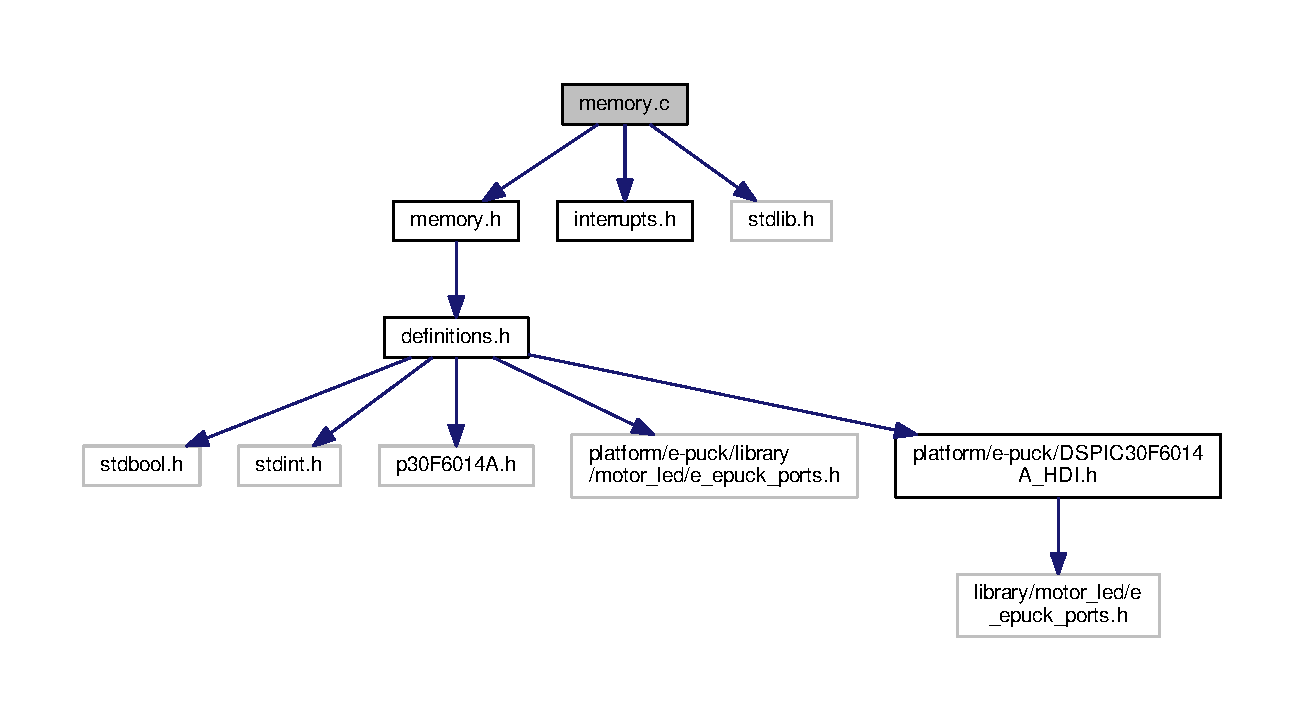
\includegraphics[width=350pt]{d1/dcd/memory_8c__incl}
\end{center}
\end{figure}
\subsection*{Functions}
\begin{DoxyCompactItemize}
\item 
void $\ast$ \hyperlink{memory_8c_aac1292ecd85eefecced84ec282250442}{Sys\+\_\+\+Malloc} (\hyperlink{definitions_8h_a05f6b0ae8f6a6e135b0e290c25fe0e4e}{uint16} length)
\item 
void \hyperlink{memory_8c_aab581d2999681f3bc60bcf46a59dfb35}{Sys\+\_\+\+Free} (void $\ast$data)
\item 
void \hyperlink{memory_8c_a0529ac1dbd051c6866093fc1493abf79}{Sys\+\_\+\+Memcpy} (void $\ast$source\+\_\+i, void $\ast$destination\+\_\+o, \hyperlink{definitions_8h_a05f6b0ae8f6a6e135b0e290c25fe0e4e}{uint16} length)
\end{DoxyCompactItemize}


\subsection{Detailed Description}
includes functions to allocate, free, and copy memory 

\begin{DoxyAuthor}{Author}
Stefan M. Trenkwalder \href{mailto:s.trenkwalder@openswarm.org}{\tt s.\+trenkwalder@openswarm.\+org} 
\end{DoxyAuthor}
\begin{DoxyVersion}{Version}
1.\+0
\end{DoxyVersion}
\begin{DoxyDate}{Date}
\{05 September 2015\}
\end{DoxyDate}
\begin{DoxyCopyright}{Copyright}
adapted Free\+B\+S\+D License (see \href{http://openswarm.org/license}{\tt http\+://openswarm.\+org/license}) 
\end{DoxyCopyright}


\subsection{Function Documentation}
\hypertarget{memory_8c_aab581d2999681f3bc60bcf46a59dfb35}{}\index{memory.\+c@{memory.\+c}!Sys\+\_\+\+Free@{Sys\+\_\+\+Free}}
\index{Sys\+\_\+\+Free@{Sys\+\_\+\+Free}!memory.\+c@{memory.\+c}}
\subsubsection[{Sys\+\_\+\+Free}]{\setlength{\rightskip}{0pt plus 5cm}void Sys\+\_\+\+Free (
\begin{DoxyParamCaption}
\item[{void $\ast$}]{data}
\end{DoxyParamCaption}
)}\label{memory_8c_aab581d2999681f3bc60bcf46a59dfb35}
Function to free memory

This Function frees dynamic allocated memory. This freeing is performed as atomic action.


\begin{DoxyParams}{Parameters}
{\em data} & pointer to memory that should be freed. \\
\hline
\end{DoxyParams}


Definition at line 45 of file memory.\+c.

\hypertarget{memory_8c_aac1292ecd85eefecced84ec282250442}{}\index{memory.\+c@{memory.\+c}!Sys\+\_\+\+Malloc@{Sys\+\_\+\+Malloc}}
\index{Sys\+\_\+\+Malloc@{Sys\+\_\+\+Malloc}!memory.\+c@{memory.\+c}}
\subsubsection[{Sys\+\_\+\+Malloc}]{\setlength{\rightskip}{0pt plus 5cm}void$\ast$ Sys\+\_\+\+Malloc (
\begin{DoxyParamCaption}
\item[{{\bf uint16}}]{length}
\end{DoxyParamCaption}
)}\label{memory_8c_aac1292ecd85eefecced84ec282250442}
Function to allocate {\bfseries length} bytes of memory

This Function allocates memory of the size {\bfseries length}. This allocation is performed as atomic action.


\begin{DoxyParams}{Parameters}
{\em length} & value how many bytes should be allocated \\
\hline
\end{DoxyParams}
\begin{DoxyReturn}{Returns}
pointer to the allocated memory 
\end{DoxyReturn}


Definition at line 26 of file memory.\+c.

\hypertarget{memory_8c_a0529ac1dbd051c6866093fc1493abf79}{}\index{memory.\+c@{memory.\+c}!Sys\+\_\+\+Memcpy@{Sys\+\_\+\+Memcpy}}
\index{Sys\+\_\+\+Memcpy@{Sys\+\_\+\+Memcpy}!memory.\+c@{memory.\+c}}
\subsubsection[{Sys\+\_\+\+Memcpy}]{\setlength{\rightskip}{0pt plus 5cm}void Sys\+\_\+\+Memcpy (
\begin{DoxyParamCaption}
\item[{void $\ast$}]{source\+\_\+i, }
\item[{void $\ast$}]{destination\+\_\+o, }
\item[{{\bf uint16}}]{length}
\end{DoxyParamCaption}
)}\label{memory_8c_a0529ac1dbd051c6866093fc1493abf79}
Function to copies memory of the size {\bfseries length} from {\bfseries source\+\_\+i} to {\bfseries destination\+\_\+o}.

Function to copies memory of the size {\bfseries length} from {\bfseries source\+\_\+i} to {\bfseries destination\+\_\+o}. This copying is performed as atomic action.


\begin{DoxyParams}{Parameters}
{\em source\+\_\+i} & pointer to the source \\
\hline
{\em destination\+\_\+o} & pointer to the destination \\
\hline
{\em length} & size of the memory that has to be copied \\
\hline
\end{DoxyParams}


Definition at line 64 of file memory.\+c.


\hypertarget{memory_8h}{}\section{memory.\+h File Reference}
\label{memory_8h}\index{memory.\+h@{memory.\+h}}


includes functions to allocate, free, and copy memory  


{\ttfamily \#include \char`\"{}definitions.\+h\char`\"{}}\\*
Include dependency graph for memory.\+h\+:\nopagebreak
\begin{figure}[H]
\begin{center}
\leavevmode
\includegraphics[width=350pt]{df/d9a/memory_8h__incl}
\end{center}
\end{figure}
This graph shows which files directly or indirectly include this file\+:\nopagebreak
\begin{figure}[H]
\begin{center}
\leavevmode
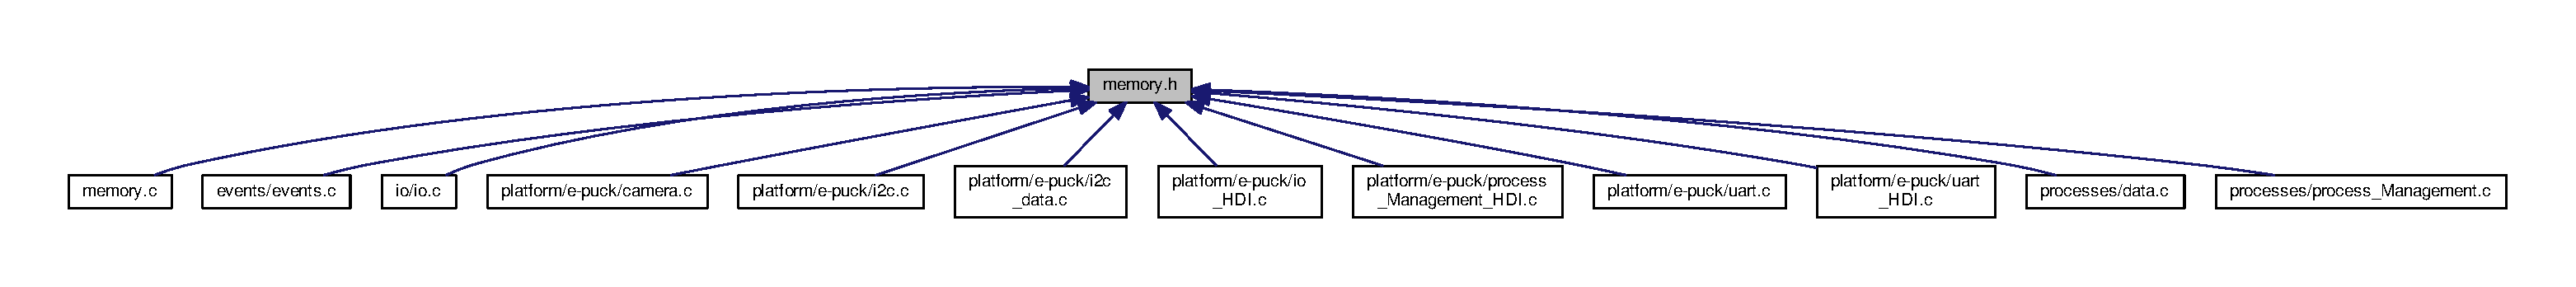
\includegraphics[width=350pt]{db/d57/memory_8h__dep__incl}
\end{center}
\end{figure}
\subsection*{Functions}
\begin{DoxyCompactItemize}
\item 
void $\ast$ \hyperlink{memory_8h_aac1292ecd85eefecced84ec282250442}{Sys\+\_\+\+Malloc} (\hyperlink{definitions_8h_a05f6b0ae8f6a6e135b0e290c25fe0e4e}{uint16} length)
\item 
void \hyperlink{memory_8h_a8f04ee5feb590ac9777b8c76c4d2cd70}{Sys\+\_\+\+Free} (void $\ast$)
\item 
void \hyperlink{memory_8h_ac496f9d5e3dc6b8644f137ad7d0e8bc4}{Sys\+\_\+\+Memcpy} (void $\ast$source, void $\ast$destination, \hyperlink{definitions_8h_a05f6b0ae8f6a6e135b0e290c25fe0e4e}{uint16} length)
\end{DoxyCompactItemize}


\subsection{Detailed Description}
includes functions to allocate, free, and copy memory 

\begin{DoxyAuthor}{Author}
Stefan M. Trenkwalder \href{mailto:s.trenkwalder@openswarm.org}{\tt s.\+trenkwalder@openswarm.\+org} 
\end{DoxyAuthor}
\begin{DoxyVersion}{Version}
1.\+0
\end{DoxyVersion}
\begin{DoxyDate}{Date}
\{05 September 2015\}
\end{DoxyDate}
\begin{DoxyCopyright}{Copyright}
adapted Free\+B\+S\+D License (see \href{http://openswarm.org/license}{\tt http\+://openswarm.\+org/license}) 
\end{DoxyCopyright}


\subsection{Function Documentation}
\hypertarget{memory_8h_a8f04ee5feb590ac9777b8c76c4d2cd70}{}\index{memory.\+h@{memory.\+h}!Sys\+\_\+\+Free@{Sys\+\_\+\+Free}}
\index{Sys\+\_\+\+Free@{Sys\+\_\+\+Free}!memory.\+h@{memory.\+h}}
\subsubsection[{Sys\+\_\+\+Free}]{\setlength{\rightskip}{0pt plus 5cm}void Sys\+\_\+\+Free (
\begin{DoxyParamCaption}
\item[{void $\ast$}]{data}
\end{DoxyParamCaption}
)}\label{memory_8h_a8f04ee5feb590ac9777b8c76c4d2cd70}
Function to free memory

This Function frees dynamic allocated memory. This freeing is performed as atomic action.


\begin{DoxyParams}{Parameters}
{\em data} & pointer to memory that should be freed. \\
\hline
\end{DoxyParams}


Definition at line 45 of file memory.\+c.

\hypertarget{memory_8h_aac1292ecd85eefecced84ec282250442}{}\index{memory.\+h@{memory.\+h}!Sys\+\_\+\+Malloc@{Sys\+\_\+\+Malloc}}
\index{Sys\+\_\+\+Malloc@{Sys\+\_\+\+Malloc}!memory.\+h@{memory.\+h}}
\subsubsection[{Sys\+\_\+\+Malloc}]{\setlength{\rightskip}{0pt plus 5cm}void$\ast$ Sys\+\_\+\+Malloc (
\begin{DoxyParamCaption}
\item[{{\bf uint16}}]{length}
\end{DoxyParamCaption}
)}\label{memory_8h_aac1292ecd85eefecced84ec282250442}
Function to allocate {\bfseries length} bytes of memory

This Function allocates memory of the size {\bfseries length}. This allocation is performed as atomic action.


\begin{DoxyParams}{Parameters}
{\em length} & value how many bytes should be allocated \\
\hline
\end{DoxyParams}
\begin{DoxyReturn}{Returns}
pointer to the allocated memory 
\end{DoxyReturn}


Definition at line 26 of file memory.\+c.

\hypertarget{memory_8h_ac496f9d5e3dc6b8644f137ad7d0e8bc4}{}\index{memory.\+h@{memory.\+h}!Sys\+\_\+\+Memcpy@{Sys\+\_\+\+Memcpy}}
\index{Sys\+\_\+\+Memcpy@{Sys\+\_\+\+Memcpy}!memory.\+h@{memory.\+h}}
\subsubsection[{Sys\+\_\+\+Memcpy}]{\setlength{\rightskip}{0pt plus 5cm}void Sys\+\_\+\+Memcpy (
\begin{DoxyParamCaption}
\item[{void $\ast$}]{source\+\_\+i, }
\item[{void $\ast$}]{destination\+\_\+o, }
\item[{{\bf uint16}}]{length}
\end{DoxyParamCaption}
)}\label{memory_8h_ac496f9d5e3dc6b8644f137ad7d0e8bc4}
Function to copies memory of the size {\bfseries length} from {\bfseries source\+\_\+i} to {\bfseries destination\+\_\+o}.

Function to copies memory of the size {\bfseries length} from {\bfseries source\+\_\+i} to {\bfseries destination\+\_\+o}. This copying is performed as atomic action.


\begin{DoxyParams}{Parameters}
{\em source\+\_\+i} & pointer to the source \\
\hline
{\em destination\+\_\+o} & pointer to the destination \\
\hline
{\em length} & size of the memory that has to be copied \\
\hline
\end{DoxyParams}


Definition at line 64 of file memory.\+c.


\hypertarget{system_8c}{}\section{system.\+c File Reference}
\label{system_8c}\index{system.\+c@{system.\+c}}


defines functions to initialise and start Open\+Swarm.  


{\ttfamily \#include \char`\"{}definitions.\+h\char`\"{}}\\*
{\ttfamily \#include \char`\"{}system.\+h\char`\"{}}\\*
{\ttfamily \#include \char`\"{}processes/system\+\_\+\+Timer.\+h\char`\"{}}\\*
{\ttfamily \#include \char`\"{}processes/scheduler.\+h\char`\"{}}\\*
{\ttfamily \#include \char`\"{}processes/process\+\_\+\+Management.\+h\char`\"{}}\\*
{\ttfamily \#include \char`\"{}platform/e-\/puck/library/motor\+\_\+led/e\+\_\+init\+\_\+port.\+h\char`\"{}}\\*
{\ttfamily \#include \char`\"{}io/io.\+h\char`\"{}}\\*
{\ttfamily \#include \char`\"{}io/io\+\_\+clock.\+h\char`\"{}}\\*
{\ttfamily \#include \char`\"{}io/e-\/puck/motors.\+h\char`\"{}}\\*
{\ttfamily \#include \char`\"{}io/e-\/puck/uart.\+h\char`\"{}}\\*
{\ttfamily \#include \char`\"{}io/e-\/puck/remote\+Control.\+h\char`\"{}}\\*
{\ttfamily \#include \char`\"{}io/e-\/puck/camera.\+h\char`\"{}}\\*
Include dependency graph for system.\+c\+:
\nopagebreak
\begin{figure}[H]
\begin{center}
\leavevmode
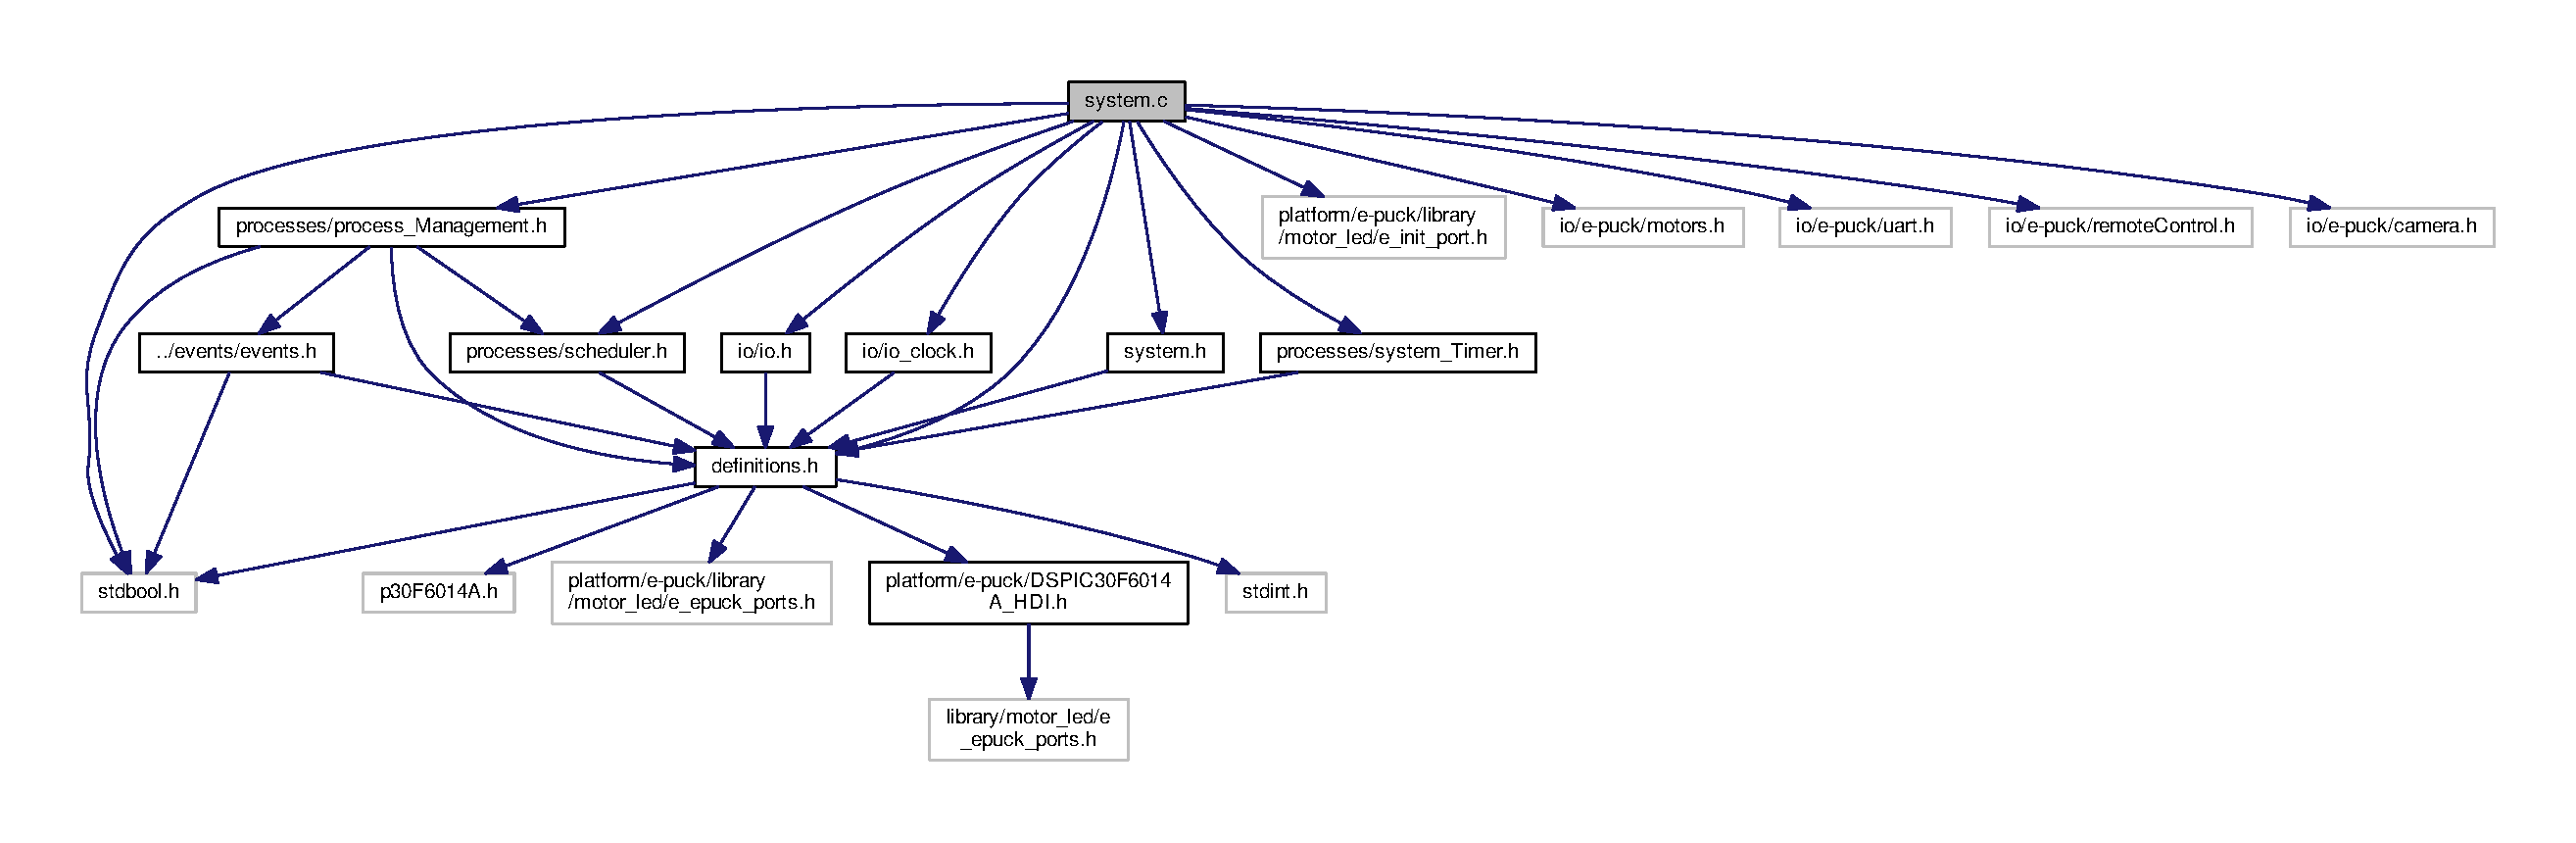
\includegraphics[width=350pt]{d3/d4a/system_8c__incl}
\end{center}
\end{figure}
\subsection*{Functions}
\begin{DoxyCompactItemize}
\item 
void \hyperlink{system_8c_a31ce626d506c2b262ecf5b23946f522f}{Sys\+\_\+\+Init\+\_\+\+Kernel} ()
\item 
void \hyperlink{system_8c_a2e15518324643f26cb240108259b30da}{Sys\+\_\+\+Start\+\_\+\+Kernel} (void)
\end{DoxyCompactItemize}


\subsection{Detailed Description}
defines functions to initialise and start Open\+Swarm. 

\begin{DoxyAuthor}{Author}
Stefan M. Trenkwalder \href{mailto:s.trenkwalder@openswarm.org}{\tt s.\+trenkwalder@openswarm.\+org} 
\end{DoxyAuthor}
\begin{DoxyVersion}{Version}
1.\+0 
\end{DoxyVersion}
\begin{DoxyDate}{Date}
2015 
\end{DoxyDate}
\begin{DoxyCopyright}{Copyright}
adapted Free\+B\+S\+D License (see \href{http://openswarm.org/license}{\tt http\+://openswarm.\+org/license})
\end{DoxyCopyright}
~\newline
 In short, Openswarm can be executed as shown in the following example 
\begin{DoxyCode}
\textcolor{preprocessor}{#include "\hyperlink{system_8h}{os/system.h}"}

\textcolor{keywordtype}{int} main(\textcolor{keywordtype}{void})\{
     \textcolor{comment}{//initialise some global or local variables}

    \hyperlink{system_8c_a31ce626d506c2b262ecf5b23946f522f}{Sys\_Init\_Kernel}();

     \textcolor{comment}{//do some preperation before executing OpenSwarm and user applications}
     
     \hyperlink{system_8c_a2e15518324643f26cb240108259b30da}{Sys\_Start\_Kernel}();      
    \textcolor{keywordflow}{while}(1)\{
        \textcolor{comment}{//do nothing}
    \}
\}
\end{DoxyCode}
 

\subsection{Function Documentation}
\hypertarget{system_8c_a31ce626d506c2b262ecf5b23946f522f}{}\index{system.\+c@{system.\+c}!Sys\+\_\+\+Init\+\_\+\+Kernel@{Sys\+\_\+\+Init\+\_\+\+Kernel}}
\index{Sys\+\_\+\+Init\+\_\+\+Kernel@{Sys\+\_\+\+Init\+\_\+\+Kernel}!system.\+c@{system.\+c}}
\subsubsection[{Sys\+\_\+\+Init\+\_\+\+Kernel}]{\setlength{\rightskip}{0pt plus 5cm}void Sys\+\_\+\+Init\+\_\+\+Kernel (
\begin{DoxyParamCaption}
\item[{void}]{}
\end{DoxyParamCaption}
)}\label{system_8c_a31ce626d506c2b262ecf5b23946f522f}
Function to initialise the hardware

This Function sets the system Timer (Timer0) and sets an scheduling algorithm. It also intitalises I/\+O devices (e.\+g. if e-\/puck is used\+: motor, U\+A\+R\+T, remote control, and camera)

\begin{DoxyPostcond}{Postcondition}
To start Open\+Swarm, \hyperlink{system_8c_a2e15518324643f26cb240108259b30da}{Sys\+\_\+\+Start\+\_\+\+Kernel()} mast be executed after the initialisation. 
\end{DoxyPostcond}
\begin{DoxyRemark}{Remarks}
Code can be executed between initialisation and start of the kernel. But, note that you can only execute code that does not depend on an active Open\+Swarm. 
\end{DoxyRemark}


Definition at line 64 of file system.\+c.

\hypertarget{system_8c_a2e15518324643f26cb240108259b30da}{}\index{system.\+c@{system.\+c}!Sys\+\_\+\+Start\+\_\+\+Kernel@{Sys\+\_\+\+Start\+\_\+\+Kernel}}
\index{Sys\+\_\+\+Start\+\_\+\+Kernel@{Sys\+\_\+\+Start\+\_\+\+Kernel}!system.\+c@{system.\+c}}
\subsubsection[{Sys\+\_\+\+Start\+\_\+\+Kernel}]{\setlength{\rightskip}{0pt plus 5cm}void Sys\+\_\+\+Start\+\_\+\+Kernel (
\begin{DoxyParamCaption}
\item[{void}]{}
\end{DoxyParamCaption}
)}\label{system_8c_a2e15518324643f26cb240108259b30da}
Function to start the the system timer

This Function starts all functions of the operating system. The system M\+U\+S\+T H\+A\+V\+E B\+E\+E\+N I\+N\+I\+T\+I\+A\+L\+I\+S\+E\+D before. \begin{DoxyPrecond}{Precondition}
System must be initialised with \hyperlink{system_8c_a31ce626d506c2b262ecf5b23946f522f}{Sys\+\_\+\+Init\+\_\+\+Kernel()}. 
\end{DoxyPrecond}
\begin{DoxyRemark}{Remarks}
Code can be executed between initialisation and start of the kernel. But, note that you can only execute code that does not depend on an active Open\+Swarm. 
\end{DoxyRemark}


Definition at line 104 of file system.\+c.


\hypertarget{system_8h}{}\section{system.\+h File Reference}
\label{system_8h}\index{system.\+h@{system.\+h}}


Initiaises and starts Open\+Swarm.  


{\ttfamily \#include \char`\"{}definitions.\+h\char`\"{}}\\*
Include dependency graph for system.\+h\+:
% FIG 0
This graph shows which files directly or indirectly include this file\+:
% FIG 1
\subsection*{Macros}
\begin{DoxyCompactItemize}
\item 
\#define \hyperlink{system_8h_aa790380273821f8d44cd42773fdd7e2a}{S\+Y\+S\+\_\+\+M\+O\+T\+O\+R\+\_\+\+U\+S\+E\+D}
\item 
\#define \hyperlink{system_8h_a7230b7bc459e2e3b1de072f9c2490d74}{S\+Y\+S\+\_\+\+U\+A\+R\+T1\+\_\+\+U\+S\+E\+D}
\item 
\#define \hyperlink{system_8h_acf553b2b5b8bb08ffc74d03b52ea68bd}{S\+Y\+S\+\_\+\+R\+E\+M\+O\+T\+E\+C\+O\+N\+T\+R\+O\+L\+\_\+\+U\+S\+E\+D}
\item 
\#define \hyperlink{system_8h_ac4c4020859ec5bd6347651b6babe7388}{S\+Y\+S\+\_\+\+C\+A\+M\+E\+R\+A\+\_\+\+U\+S\+E\+D}
\end{DoxyCompactItemize}
\subsection*{Functions}
\begin{DoxyCompactItemize}
\item 
void \hyperlink{system_8h_a9cfaef0a7af7eea16e065c481662eaa4}{Sys\+\_\+\+Init\+\_\+\+Kernel} (void)
\item 
void \hyperlink{system_8h_a2e15518324643f26cb240108259b30da}{Sys\+\_\+\+Start\+\_\+\+Kernel} (void)
\end{DoxyCompactItemize}


\subsection{Detailed Description}
Initiaises and starts Open\+Swarm. 

\begin{DoxyAuthor}{Author}
Stefan M. Trenkwalder \href{mailto:s.trenkwalder@openswarm.org}{\tt s.\+trenkwalder@openswarm.\+org} 
\end{DoxyAuthor}
\begin{DoxyVersion}{Version}
1.\+0
\end{DoxyVersion}
\begin{DoxyDate}{Date}
\{07 July 2014\} 
\end{DoxyDate}


\subsection{Macro Definition Documentation}
\hypertarget{system_8h_ac4c4020859ec5bd6347651b6babe7388}{}\index{system.\+h@{system.\+h}!S\+Y\+S\+\_\+\+C\+A\+M\+E\+R\+A\+\_\+\+U\+S\+E\+D@{S\+Y\+S\+\_\+\+C\+A\+M\+E\+R\+A\+\_\+\+U\+S\+E\+D}}
\index{S\+Y\+S\+\_\+\+C\+A\+M\+E\+R\+A\+\_\+\+U\+S\+E\+D@{S\+Y\+S\+\_\+\+C\+A\+M\+E\+R\+A\+\_\+\+U\+S\+E\+D}!system.\+h@{system.\+h}}
\subsubsection[{S\+Y\+S\+\_\+\+C\+A\+M\+E\+R\+A\+\_\+\+U\+S\+E\+D}]{\setlength{\rightskip}{0pt plus 5cm}\#define S\+Y\+S\+\_\+\+C\+A\+M\+E\+R\+A\+\_\+\+U\+S\+E\+D}\label{system_8h_ac4c4020859ec5bd6347651b6babe7388}
Define this preprocessor symbol to use the camera 

Definition at line 88 of file system.\+h.

\hypertarget{system_8h_aa790380273821f8d44cd42773fdd7e2a}{}\index{system.\+h@{system.\+h}!S\+Y\+S\+\_\+\+M\+O\+T\+O\+R\+\_\+\+U\+S\+E\+D@{S\+Y\+S\+\_\+\+M\+O\+T\+O\+R\+\_\+\+U\+S\+E\+D}}
\index{S\+Y\+S\+\_\+\+M\+O\+T\+O\+R\+\_\+\+U\+S\+E\+D@{S\+Y\+S\+\_\+\+M\+O\+T\+O\+R\+\_\+\+U\+S\+E\+D}!system.\+h@{system.\+h}}
\subsubsection[{S\+Y\+S\+\_\+\+M\+O\+T\+O\+R\+\_\+\+U\+S\+E\+D}]{\setlength{\rightskip}{0pt plus 5cm}\#define S\+Y\+S\+\_\+\+M\+O\+T\+O\+R\+\_\+\+U\+S\+E\+D}\label{system_8h_aa790380273821f8d44cd42773fdd7e2a}
Define this preprocessor symbol to use motors 

Definition at line 85 of file system.\+h.

\hypertarget{system_8h_acf553b2b5b8bb08ffc74d03b52ea68bd}{}\index{system.\+h@{system.\+h}!S\+Y\+S\+\_\+\+R\+E\+M\+O\+T\+E\+C\+O\+N\+T\+R\+O\+L\+\_\+\+U\+S\+E\+D@{S\+Y\+S\+\_\+\+R\+E\+M\+O\+T\+E\+C\+O\+N\+T\+R\+O\+L\+\_\+\+U\+S\+E\+D}}
\index{S\+Y\+S\+\_\+\+R\+E\+M\+O\+T\+E\+C\+O\+N\+T\+R\+O\+L\+\_\+\+U\+S\+E\+D@{S\+Y\+S\+\_\+\+R\+E\+M\+O\+T\+E\+C\+O\+N\+T\+R\+O\+L\+\_\+\+U\+S\+E\+D}!system.\+h@{system.\+h}}
\subsubsection[{S\+Y\+S\+\_\+\+R\+E\+M\+O\+T\+E\+C\+O\+N\+T\+R\+O\+L\+\_\+\+U\+S\+E\+D}]{\setlength{\rightskip}{0pt plus 5cm}\#define S\+Y\+S\+\_\+\+R\+E\+M\+O\+T\+E\+C\+O\+N\+T\+R\+O\+L\+\_\+\+U\+S\+E\+D}\label{system_8h_acf553b2b5b8bb08ffc74d03b52ea68bd}
Define this preprocessor symbol to receive remote control signals 

Definition at line 87 of file system.\+h.

\hypertarget{system_8h_a7230b7bc459e2e3b1de072f9c2490d74}{}\index{system.\+h@{system.\+h}!S\+Y\+S\+\_\+\+U\+A\+R\+T1\+\_\+\+U\+S\+E\+D@{S\+Y\+S\+\_\+\+U\+A\+R\+T1\+\_\+\+U\+S\+E\+D}}
\index{S\+Y\+S\+\_\+\+U\+A\+R\+T1\+\_\+\+U\+S\+E\+D@{S\+Y\+S\+\_\+\+U\+A\+R\+T1\+\_\+\+U\+S\+E\+D}!system.\+h@{system.\+h}}
\subsubsection[{S\+Y\+S\+\_\+\+U\+A\+R\+T1\+\_\+\+U\+S\+E\+D}]{\setlength{\rightskip}{0pt plus 5cm}\#define S\+Y\+S\+\_\+\+U\+A\+R\+T1\+\_\+\+U\+S\+E\+D}\label{system_8h_a7230b7bc459e2e3b1de072f9c2490d74}
Define this preprocessor symbol to use U\+A\+R\+T1 

Definition at line 86 of file system.\+h.



\subsection{Function Documentation}
\hypertarget{system_8h_a9cfaef0a7af7eea16e065c481662eaa4}{}\index{system.\+h@{system.\+h}!Sys\+\_\+\+Init\+\_\+\+Kernel@{Sys\+\_\+\+Init\+\_\+\+Kernel}}
\index{Sys\+\_\+\+Init\+\_\+\+Kernel@{Sys\+\_\+\+Init\+\_\+\+Kernel}!system.\+h@{system.\+h}}
\subsubsection[{Sys\+\_\+\+Init\+\_\+\+Kernel}]{\setlength{\rightskip}{0pt plus 5cm}void Sys\+\_\+\+Init\+\_\+\+Kernel (
\begin{DoxyParamCaption}
\item[{void}]{}
\end{DoxyParamCaption}
)}\label{system_8h_a9cfaef0a7af7eea16e065c481662eaa4}
Function to initialise the hardware

This Function sets the system Timer (Timer0) and sets an scheduling algorithm. It also intitalises I/\+O devices (e.\+g. if e-\/puck is used\+: motor, U\+A\+R\+T, remote control, and camera)

\begin{DoxyPostcond}{Postcondition}
To start Open\+Swarm, \hyperlink{system_8c_a2e15518324643f26cb240108259b30da}{Sys\+\_\+\+Start\+\_\+\+Kernel()} mast be executed after the initialisation. 
\end{DoxyPostcond}
\begin{DoxyRemark}{Remarks}
Code can be executed between initialisation and start of the kernel. But, note that you can only execute code that does not depend on an active Open\+Swarm. 
\end{DoxyRemark}

\begin{DoxyParams}{Parameters}
{\em void} & \\
\hline
\end{DoxyParams}
\begin{DoxyReturn}{Returns}
void 
\end{DoxyReturn}


Definition at line 64 of file system.\+c.

\hypertarget{system_8h_a2e15518324643f26cb240108259b30da}{}\index{system.\+h@{system.\+h}!Sys\+\_\+\+Start\+\_\+\+Kernel@{Sys\+\_\+\+Start\+\_\+\+Kernel}}
\index{Sys\+\_\+\+Start\+\_\+\+Kernel@{Sys\+\_\+\+Start\+\_\+\+Kernel}!system.\+h@{system.\+h}}
\subsubsection[{Sys\+\_\+\+Start\+\_\+\+Kernel}]{\setlength{\rightskip}{0pt plus 5cm}void Sys\+\_\+\+Start\+\_\+\+Kernel (
\begin{DoxyParamCaption}
\item[{void}]{}
\end{DoxyParamCaption}
)}\label{system_8h_a2e15518324643f26cb240108259b30da}
Function to start the the system timer

This Function starts all functions of the operating system. The system M\+U\+S\+T H\+A\+V\+E B\+E\+E\+N I\+N\+I\+T\+I\+A\+L\+I\+S\+E\+D before. \begin{DoxyPrecond}{Precondition}
System must be initialised with \hyperlink{system_8c_a31ce626d506c2b262ecf5b23946f522f}{Sys\+\_\+\+Init\+\_\+\+Kernel()}. 
\end{DoxyPrecond}
\begin{DoxyRemark}{Remarks}
Code can be executed between initialisation and start of the kernel. But, note that you can only execute code that does not depend on an active Open\+Swarm. 
\end{DoxyRemark}

\begin{DoxyParams}{Parameters}
{\em void} & \\
\hline
\end{DoxyParams}
\begin{DoxyReturn}{Returns}
void 
\end{DoxyReturn}


Definition at line 106 of file system.\+c.


%--- End generated contents ---

% Index
\backmatter
\newpage
\phantomsection
\clearemptydoublepage
\addcontentsline{toc}{chapter}{Index}
\printindex

\end{document}
